\chapter{How Biology Differs from Engineering}
\label{ch:bio-vs-eng}

\epigraph{%
  Nature does not build machines. It grows organisms.
  The engineer's model of the body is a useful fiction---but it is fiction.
}{--- Adapted from D'Arcy Wentworth Thompson}

\vspace{0.5cm}

\section{The Rigid-Body Assumption and Its Limits}

Every model in Volumes~0--II rested on a fundamental assumption: the moving
system consists of \emph{rigid bodies} connected by \emph{ideal joints}. A rigid body
has a fixed mass distribution; its shape does not change under load. An ideal revolute
joint constrains five of six relative degrees of freedom, permitting only rotation
about a single axis. These assumptions are extraordinarily productive for engineering
systems---robot arms, spacecraft, mechanisms---where components are designed to
approximate rigidity.

In biological systems, these assumptions fail at every level:

\begin{enumerate}[label=(\roman*)]
  \item \textbf{Bones are not rigid.} Long bones (femur, humerus, tibia) have measurable
        compliance under dynamic loading. A golf club shaft deflects by several centimeters
        and several degrees during a swing; a human femur deflects by millimeters during
        running. The deflection is small in absolute terms but can have significant effects
        on end-effector accuracy.

  \item \textbf{Joints are not revolutes.} The knee, for example, combines rolling,
        sliding, and rotation in a coupled manner that changes with flexion angle. The
        glenohumeral (shoulder) joint permits motion in three rotational axes but also
        allows several millimeters of translation. The intervertebral joints of the spine
        have six degrees of freedom each, all coupled through the disc and ligament
        mechanics.

  \item \textbf{Actuators are not torque sources.} Muscles produce force, not torque.
        Force is generated through the contraction of sarcomeres, transmitted through
        tendons, and converted to joint torque via moment arms that vary with joint angle.
        The force a muscle can produce depends on its length, its contraction velocity,
        and its activation history---dependencies that have no analog in electric motors.

  \item \textbf{Sensors are noisy, delayed, and multimodal.} Proprioceptors (muscle
        spindles, Golgi tendon organs, joint receptors) provide state information with
        significant noise and delays of 30--100~ms. The central nervous system must
        fuse information from proprioceptive, visual, and vestibular sources to estimate
        the body's state.

  \item \textbf{The system adapts.} Unlike a robot, the human body changes over
        time---muscles fatigue, connective tissue remodels, neural pathways strengthen
        or weaken. A complete model must account for adaptation on timescales from seconds
        (fatigue) to years (training).
\end{enumerate}

\begin{comparison}{The Fundamental Differences}{rigid-vs-bio}
\begin{center}
\renewcommand{\arraystretch}{1.3}
\begin{tabular}{@{}lll@{}}
\toprule
\textbf{Property} & \textbf{Engineering System} & \textbf{Biological System} \\
\midrule
Links & Rigid bodies & Viscoelastic, deformable \\
Joints & 1-DOF revolute/prismatic & Multi-DOF, coupled, with laxity \\
Actuators & Motors (torque on command) & Muscles (force via excitation-contraction) \\
Transmission & Gears, belts (rigid) & Tendons (elastic, energy-storing) \\
Sensors & Encoders (precise, fast) & Proprioceptors (noisy, delayed) \\
Parameters & Fixed (by design) & Variable (fatigue, adaptation, growth) \\
Redundancy & Minimal (cost-driven) & Massive (evolution-driven) \\
Failure mode & Brittle (sudden) & Graceful (degradation) \\
\bottomrule
\end{tabular}
\end{center}
\end{comparison}

These differences reflect fundamentally distinct design philosophies. Engineering systems are designed
for precise, repeatable control of pre-specified outputs. Biological systems are evolved for robustness,
adaptability, and efficiency under uncertain conditions. Neither approach is superior; rather, they
optimize for different objectives. Understanding which differences are essential for your particular
biomechanical question is crucial for successful modeling.

\begin{center}
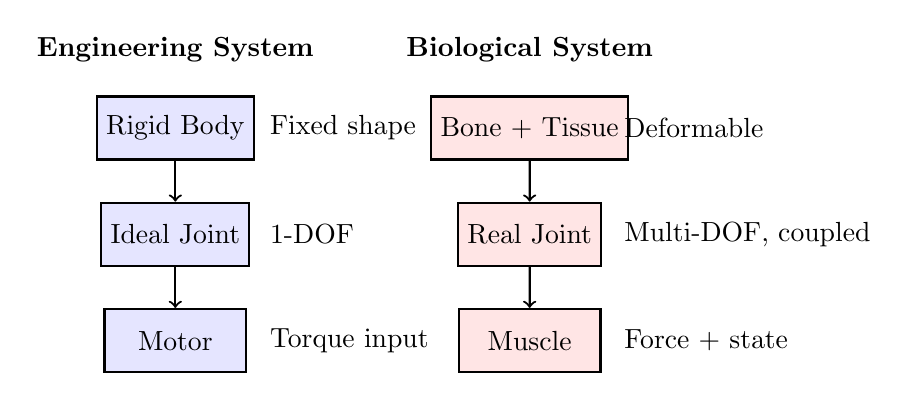
\begin{tikzpicture}[scale=0.9, node distance=2.5cm]
  % Left side: Engineering system
  \node[rectangle, draw, thick, minimum width=1.8cm, minimum height=0.8cm, fill=blue!10] (eng-body) at (0, 0) {Rigid Body};
  \node[rectangle, draw, thick, minimum width=1.8cm, minimum height=0.8cm, fill=blue!10] (eng-joint) at (0, -1.5) {Ideal Joint};
  \node[rectangle, draw, thick, minimum width=1.8cm, minimum height=0.8cm, fill=blue!10] (eng-motor) at (0, -3) {Motor};

  \draw[->, thick] (eng-body) -- (eng-joint);
  \draw[->, thick] (eng-joint) -- (eng-motor);

  \node[above] at (0, 0.8) {\textbf{Engineering System}};
  \node[right] at (1.2, 0) {Fixed shape};
  \node[right] at (1.2, -1.5) {1-DOF};
  \node[right] at (1.2, -3) {Torque input};

  % Right side: Biological system
  \node[rectangle, draw, thick, minimum width=1.8cm, minimum height=0.8cm, fill=red!10] (bio-body) at (5, 0) {Bone + Tissue};
  \node[rectangle, draw, thick, minimum width=1.8cm, minimum height=0.8cm, fill=red!10] (bio-joint) at (5, -1.5) {Real Joint};
  \node[rectangle, draw, thick, minimum width=1.8cm, minimum height=0.8cm, fill=red!10] (bio-muscle) at (5, -3) {Muscle};

  \draw[->, thick] (bio-body) -- (bio-joint);
  \draw[->, thick] (bio-joint) -- (bio-muscle);

  \node[above] at (5, 0.8) {\textbf{Biological System}};
  \node[right] at (6.2, 0) {Deformable};
  \node[right] at (6.2, -1.5) {Multi-DOF, coupled};
  \node[right] at (6.2, -3) {Force + state};
\end{tikzpicture}
\end{center}

\section{Why the Differences Matter for Control}

The differences enumerated above are not merely academic. They fundamentally change
the control problem in ways that Volumes~I and~II must now accommodate.

\subsection{Compliance Creates Hidden Dynamics}

When a link is compliant, its deformation adds internal degrees of freedom to the system.
A golf club shaft, modeled as rigid, has one degree of freedom (the grip angle). Modeled
as a flexible beam, it has \emph{infinitely many} degrees of freedom, though practical
models truncate to the first 2--3 bending modes. The equation of motion becomes:
\begin{equation}
  \underbrace{M(\bm{q})\ddot{\bm{q}} + C(\bm{q},\dot{\bm{q}})\dot{\bm{q}} + g(\bm{q})}_{\text{rigid-body dynamics}}
  + \underbrace{K_{\text{stiff}} \bm{q}_{\text{flex}} + D_{\text{damp}} \dot{\bm{q}}_{\text{flex}}}_{\text{flexibility terms}}
  = \bm{\tau},
  \label{eq:ch1:flexible-eom}
\end{equation}
where $\bm{q}_{\text{flex}}$ represents the modal coordinates of the flexible modes,
$K_{\text{stiff}}$ is the stiffness matrix, and $D_{\text{damp}}$ is the structural
damping matrix.

\begin{principle}{The Timescale Separation Principle}{timescale}
  In many biological systems, the flexible dynamics are \emph{fast} relative to the
  rigid-body dynamics. If the natural frequency of the flexible modes is much higher
  than the bandwidth of the controller, the flexibility can be modeled as a
  quasi-static compliance rather than a dynamic mode. Specifically, if the $k$-th
  flexible mode has natural frequency $\omega_k$ and the controller bandwidth is
  $\omega_c$, then:
  \begin{itemize}
    \item $\omega_k \gg \omega_c$: quasi-static (flexibility ``follows'' the rigid motion)
    \item $\omega_k \approx \omega_c$: resonance risk (flexibility must be modeled dynamically)
    \item $\omega_k \ll \omega_c$: the system is effectively another rigid body (the
          flexible mode is so slow it acts like a separate DOF)
  \end{itemize}
\end{principle}

The timescale separation principle is critical for model selection. For different body
regions and different movement speeds, the applicability of the rigid-body approximation varies.
For the human body during locomotion, empirical measurements suggest that long bones have natural
frequencies sufficiently high that the rigid-body assumption is justified. For the spine and
soft tissues, particularly during rapid movements, the separation is less clean, and dynamic
flexibility effects may contribute meaningfully to the system behavior. The choice of whether to
include flexibility as explicit state variables or treat it as a quasi-static effect should be
guided by both the timescale analysis above and by quantitative comparison of model predictions
to experimental data.

\subsection{Muscle Force Production Is State-Dependent}

The most profound difference between engineered and biological actuators is that muscle
force depends on the \emph{state of the muscle itself}. An electric motor produces torque
proportional to current, regardless of shaft angle or angular velocity (to first
approximation). A muscle's maximum force depends on:

\begin{enumerate}
  \item \textbf{Muscle length} (force-length relationship): maximum isometric force
        occurs at an intermediate ``optimal'' length $\ell_0$, with force decreasing
        at shorter and longer lengths.
  \item \textbf{Contraction velocity} (force-velocity relationship): concentric
        (shortening) contractions produce less force at higher velocities; eccentric
        (lengthening) contractions can produce forces exceeding the maximum isometric
        force by 50--80\%.
  \item \textbf{Activation level}: the fraction of motor units recruited and their
        firing rates, which follows its own first-order dynamics with time constants
        of 10--50~ms for activation and 40--200~ms for deactivation.
\end{enumerate}

The combined force production model (Hill model, Chapter~3) is:
\begin{equation}
  F_{\text{muscle}} = a(t) \cdot f_L(\tilde{\ell}) \cdot f_V(\tilde{v}) \cdot F_0
  + f_{\text{PE}}(\tilde{\ell}),
  \label{eq:ch1:hill-overview}
\end{equation}
where $a(t) \in [0,1]$ is the activation level, $f_L$ and $f_V$ are the normalized
force-length and force-velocity curves, $F_0$ is the maximum isometric force,
$\tilde{\ell} = \ell/\ell_0$ and $\tilde{v} = v/v_0$ are normalized length and velocity,
and $f_{\text{PE}}$ is the passive elastic force.

\begin{principle}{Force-Velocity Asymmetry in Multi-Joint Tasks}{fv-asymmetry-task}
  In any task where joints undergo different phases of contraction (some concentric,
  others eccentric), the force-velocity relationship creates an asymmetry in joint
  torque capacity. This asymmetry can be quantified through the Hill force-velocity
  function applied to each muscle group. The engineering consequence is that a model
  assuming constant or task-invariant joint torque limits systematically misrepresents
  the instantaneous torque capacity of biological joints, particularly during rapid
  multi-joint movements.
\end{principle}

\subsection{Redundancy Is a Feature, Not a Bug}

The human body has approximately 630 skeletal muscles controlling approximately 240
joint degrees of freedom. Even for a simple task like reaching for a cup (which
constrains only 6 degrees of freedom---3 position + 3 orientation of the hand),
there are vastly more muscles and joints than constraints. This \emph{motor redundancy}
means that infinitely many muscle activation patterns can produce the same hand
trajectory.

In engineering, redundancy is minimized to reduce cost. In biology, redundancy is
\emph{the solution to robustness}:

\begin{itemize}
  \item If one muscle is fatigued, others can compensate.
  \item If a joint is injured, the task can be accomplished through alternative
        kinematic chains.
  \item Variability in execution---far from being noise to be eliminated---allows
        the system to explore the space of solutions and find robust attractors
        (see Volume~IV for the motor control implications).
\end{itemize}

This connects directly to the \emph{uncontrolled manifold hypothesis}
\cite{ScholzSchoner1999}: task-irrelevant variability is not suppressed by the
nervous system, only task-relevant variability is. The biological control
system does not solve the full redundancy problem; it projects the problem
onto the task-relevant subspace.

\section{Modeling Strategies}

Given the complexity of biological systems, modelers must choose their level of
abstraction carefully. Three broad strategies exist, listed in order of increasing
fidelity:

\subsection{Strategy 1: Rigid-Body with Torque Actuators}

The simplest approach: treat biological segments as rigid bodies and joints as
ideal revolutes, with ``joint torques'' as the control input. This is the model
assumed throughout Volumes~I--II.

\textbf{Advantages:}
\begin{itemize}
  \item Mathematically tractable (standard Lagrangian mechanics)
  \item Sufficient for gross motion analysis
  \item Compatible with all control-theoretic tools from Volumes~I--II
\end{itemize}

\textbf{Limitations:}
\begin{itemize}
  \item Cannot predict muscle activation patterns
  \item Cannot account for muscle force-length-velocity constraints
  \item Cannot predict injury mechanisms
  \item Cannot capture bi-articular muscle effects
\end{itemize}

\textbf{When to use:} Trajectory optimization, gross motion planning, initial
controller design.

\subsection{Strategy 2: Rigid-Body with Muscle Actuators}

Replace torque actuators with Hill-type muscle models (Chapter~3). Joint torques
become \emph{outputs} of the model, computed from muscle forces and moment arms:
\begin{equation}
  \tau_j = \sum_{i \in \mathcal{M}_j} r_{ij}(\bm{q}) \cdot F_{\text{muscle},i},
  \label{eq:ch1:muscle-torque}
\end{equation}
where $\mathcal{M}_j$ is the set of muscles crossing joint $j$ and $r_{ij}(\bm{q})$
is the moment arm of muscle $i$ about joint $j$.

\textbf{Advantages:}
\begin{itemize}
  \item Predicts muscle activation patterns
  \item Captures force-length-velocity constraints
  \item Accounts for bi-articular coupling
  \item Can predict co-contraction and joint stiffness modulation
\end{itemize}

\textbf{Limitations:}
\begin{itemize}
  \item Significant increase in model complexity (typically 2--3 states per muscle)
  \item Muscle parameters are difficult to measure in vivo
  \item Still assumes rigid segments and ideal joints
\end{itemize}

\textbf{When to use:} Detailed motion analysis, muscle force prediction, clinical
biomechanics, prosthetic design.

\subsection{Strategy 3: Flexible Multi-Body with Muscle Actuators}

The most complete approach: flexible bodies (beam or FEM models) with muscle
actuators and realistic joint models. This is the domain of software platforms
like OpenSim and AnyBody.

\textbf{Advantages:}
\begin{itemize}
  \item Highest fidelity
  \item Can predict stress distributions in bones and soft tissues
  \item Can capture coupled joint kinematics
\end{itemize}

\textbf{Limitations:}
\begin{itemize}
  \item Computationally expensive
  \item Many parameters, often poorly known
  \item Too complex for real-time control applications
\end{itemize}

\textbf{When to use:} Injury prediction, surgical planning, detailed structural
analysis.

\begin{lstlisting}[language=Python, caption={Choosing a modeling strategy based on application requirements.}]
import numpy as np

def select_modeling_strategy(
    need_muscle_forces: bool,
    need_tissue_stress: bool,
    real_time_required: bool,
    n_dof: int
) -> str:
    """Select the appropriate biomechanical modeling strategy.

    Parameters
    ----------
    need_muscle_forces : bool
        Whether individual muscle forces are needed.
    need_tissue_stress : bool
        Whether stress/strain in tissues is needed.
    real_time_required : bool
        Whether the model must run in real-time.
    n_dof : int
        Number of degrees of freedom in the model.

    Returns
    -------
    str
        Recommended modeling strategy.
    """
    if need_tissue_stress:
        return "Strategy 3: Flexible multi-body + muscles (OpenSim/FEM)"
    elif need_muscle_forces:
        if real_time_required and n_dof > 20:
            return ("Strategy 2 (reduced): Muscle model with "
                    "synergy-based dimensionality reduction")
        return "Strategy 2: Rigid-body + Hill-type muscles (OpenSim)"
    else:
        if real_time_required:
            return "Strategy 1: Rigid-body + torque actuators (fastest)"
        return ("Strategy 1 or 2 depending on available data "
                "and analysis goals")
\end{lstlisting}

\section{A Quantitative Tour of the Human Body}

Before diving into the detailed modeling chapters, we present a quantitative overview
of the key biomechanical properties that any model must capture. All values in this
section are drawn from published anthropometric studies and are cited in the relevant
subsections.

\subsection{Segment Inertial Properties}

The human body can be decomposed into 15--20 segments for modeling purposes. The
standard segmentation and mass fractions are based on cadaver studies, most notably
those of Dempster (1955), updated by de~Leva (1996) \cite{deLeva1996}.

\begin{center}
\renewcommand{\arraystretch}{1.2}
\begin{tabular}{@{}lccc@{}}
\toprule
\textbf{Segment} & \textbf{Mass (\% body)} & \textbf{Length (cm, 180cm male)} & \textbf{CoM (\% proximal)} \\
\midrule
Head + neck & 8.1 & 25.4 & 50.0 \\
Trunk & 49.7 & 53.0 & 44.9 \\
Upper arm & 2.7 & 28.2 & 57.7 \\
Forearm & 1.6 & 26.9 & 45.7 \\
Hand & 0.6 & 19.0 & 36.2 \\
Thigh & 14.2 & 42.2 & 40.9 \\
Shank & 4.3 & 43.4 & 43.4 \\
Foot & 1.4 & 25.8 & 44.2 \\
\bottomrule
\end{tabular}
\end{center}

\begin{lstlisting}[language=Python, caption={Computing segment inertial properties from body measurements.}]
import numpy as np
from dataclasses import dataclass

@dataclass
class SegmentProperties:
    """Inertial properties of a body segment."""
    name: str
    mass: float          # kg
    length: float        # m
    com_proximal: float  # fraction from proximal end
    I_com: float         # moment of inertia about CoM, kg*m^2

def de_leva_male_segments(
    body_mass: float,
    body_height: float
) -> list[SegmentProperties]:
    """Compute segment properties using de Leva (1996) regression.

    Parameters
    ----------
    body_mass : float
        Total body mass in kg.
    body_height : float
        Total body height in m.

    Returns
    -------
    list[SegmentProperties]
        List of segment inertial properties.

    References
    ----------
    de Leva, P. (1996). Adjustments to Zatsiorsky-Seluyanov's
    segment inertia parameters. J. Biomechanics, 29(9), 1223-1230.
    """
    # Mass fractions, length fractions, CoM fractions, RoG fractions
    # (proximal reference, male data from de Leva 1996 Table 4)
    data = {
        'head_neck':  (0.0810, 0.1414, 0.5002, 0.3030),
        'trunk':      (0.4970, 0.2946, 0.4486, 0.3271),
        'upper_arm':  (0.0271, 0.1566, 0.5772, 0.2850),
        'forearm':    (0.0162, 0.1494, 0.4574, 0.2760),
        'hand':       (0.0061, 0.1057, 0.3624, 0.2880),
        'thigh':      (0.1416, 0.2321, 0.4095, 0.3290),
        'shank':      (0.0433, 0.2411, 0.4340, 0.2550),
        'foot':       (0.0137, 0.1527, 0.4415, 0.2570),
    }

    segments = []
    for name, (mass_frac, len_frac, com_frac, rog_frac) in data.items():
        seg_mass = mass_frac * body_mass
        seg_length = len_frac * body_height
        seg_com = com_frac
        # Moment of inertia: I = m * (rog * length)^2
        seg_I = seg_mass * (rog_frac * seg_length) ** 2
        segments.append(SegmentProperties(
            name=name, mass=seg_mass, length=seg_length,
            com_proximal=seg_com, I_com=seg_I
        ))

    return segments


# Example usage
if __name__ == "__main__":
    segments = de_leva_male_segments(body_mass=80.0, body_height=1.80)
    print(f"{'Segment':<15} {'Mass (kg)':>10} {'Length (m)':>10} "
          f"{'I_com (kg*m^2)':>14}")
    print("-" * 52)
    for seg in segments:
        print(f"{seg.name:<15} {seg.mass:>10.2f} {seg.length:>10.3f} "
              f"{seg.I_com:>14.4f}")
\end{lstlisting}

\subsection{Joint Ranges of Motion}

Each joint has characteristic ranges of motion that define the configuration space
$\mathcal{Q}$ of the body. Unlike robot joints, which can be modeled as
$q_i \in [\underline{q}_i, \overline{q}_i]$, biological joints have \emph{soft limits}:
resistance increases gradually as the joint approaches its anatomical limit, governed
by the elasticity of ligaments and joint capsule.

\subsection{Muscle Properties}

The human body contains approximately 630 skeletal muscles. Each is characterized by
several anatomical and physiological parameters that determine its force production capacity.
The standard parameters are:

\begin{itemize}
  \item \textbf{Maximum isometric force} $F_0$: the force a muscle produces at optimal
        length with full activation and zero velocity. Values vary widely by muscle size,
        composition, and fiber type.
  \item \textbf{Optimal fiber length} $\ell_0$: the length at which maximum isometric force
        is produced, determined by the sarcomere length ($\sim$2.6 $\mu$m per sarcomere at
        $\ell_0$).
  \item \textbf{Maximum contraction velocity} $v_0$: the velocity at which a muscle produces
        zero force under concentric contraction, measured in fiber lengths per second (typically
        $0.5$--$3$ fiber lengths per second for slow-twitch fibers, $5$--$15$ for fast-twitch).
  \item \textbf{Tendon slack length} $\ell_T^s$: the length of the tendon at which it begins to
        transmit force (below this length, the tendon is slack and carries no load).
  \item \textbf{Pennation angle} $\alpha_0$: the angle between muscle fiber direction and the
        tendon line of action at optimal fiber length. Ranges from approximately $0^\circ$ for
        parallel-fibered muscles to $30^\circ$ or more for highly pennate muscles.
\end{itemize}

These properties have been systematically measured and catalogued through:
\begin{enumerate}
  \item \cite{Zajac1989}: foundational review of muscle mechanics and parameter estimation
  \item \cite{Delp2007}: comprehensive OpenSim musculoskeletal model with measured parameters for major muscles
  \item \cite{Arnold2010}: detailed muscle morphometry from imaging and cadaver studies
\end{enumerate}

Values for specific muscles are provided in software platforms (OpenSim 4.x, AnyBody) and should
be obtained from published measurements rather than estimated.

\section{Connecting to the Control Framework}

Despite the added complexity, the control framework of Volumes~I and~II remains
applicable---with modifications. The key insight is:

\begin{principle}{The Extended Affine Structure}{affine-bio}
  A musculoskeletal system can be written in control-affine form as
  \begin{equation}
    \dot{\state} = f(\state) + G(\state) \bm{u},
    \label{eq:ch1:affine-bio}
  \end{equation}
  where the state $\state$ now includes muscle states (activation, fiber length)
  in addition to joint coordinates and velocities, the drift field $f$ includes
  passive muscle and tendon forces, and $G(\state)$ maps neural excitation signals
  $\bm{u}$ to state derivatives through the muscle activation and contraction dynamics.
  The dimensions expand---from $2n$ states with $n$ joints and $m$ torque actuators
  to $2n + 2p$ states with $p$ muscles---but the \emph{structure} of the problem
  (drift + control) is preserved.
\end{principle}

\begin{remark}{Dimensional Expansion of the State Space}{expanded_manifold}
  Recall from Volumes~0 and~I that the state manifold $\mathcal{M}$ has dimension $2n$ for a system
  with $n$ joint degrees of freedom (tracking positions and velocities). When muscles are included,
  the state space expands: for each of $p$ muscles, we add two dimensions to track activation $a_i$
  and fiber length $\ell_i^M$, yielding a state space of dimension $2n + 2p$. The system still evolves
  according to $\dot{\state} = f(\state) + G(\state) \bm{u}$, but the ambient manifold is now much
  higher-dimensional. All differential geometry tools (Lie brackets, contraction metrics, etc.)\ from
  Volumes~I--II apply without modification, though computational complexity scales with dimension.
\end{remark}

This means:
\begin{itemize}
  \item The tangent-space analysis of Volume~I applies to the expanded state space
  \item Contraction theory (Volume~I, Chapter~4) can assess stability of the
        muscle-driven system
  \item Trajectory optimization (Volume~I, Chapter~5) extends to find optimal
        neural excitation patterns
  \item The counterfactual analysis (Volume~I, Chapter~7) can distinguish which
        aspects of muscle force production contribute to the motion
\end{itemize}

The challenge is \emph{dimensionality}: a 20-DOF body with 100 muscles has a
state space of dimension $2 \times 20 + 2 \times 100 = 240$. This is precisely
the ``curse of dimensionality'' that Volume~IV addresses through the lens of
motor control and neural architecture.

\section*{Exercises}

\begin{enumerate}
  \item \textbf{Segment Properties.}
        Using the \texttt{de\_leva\_male\_segments()} function, compute the total
        mass and center of mass of a 75-kg, 1.75-m male in the anatomical position.
        Verify that the total mass sums to the body mass.

  \item \textbf{Compliance Effects.}
        A golf club shaft has a first bending mode at approximately 5~Hz. If the
        downswing takes 0.25~s, how many oscillation cycles of the shaft occur during
        the downswing? Does the timescale separation principle (Principle~\ref{princ:timescale})
        justify neglecting shaft flexibility? Discuss.

  \item \textbf{Redundancy Quantification.}
        A planar model of the arm has 3 joints (shoulder, elbow, wrist) and 6 muscles.
        If the task is to place the fingertip at a given $(x, y)$ position, what is the
        dimension of the null space? How many independent muscle patterns produce the same
        fingertip position?

  \item \textbf{Force-Velocity Impact.}
        During a golf downswing, the wrist extensors lengthen at approximately 5 fiber
        lengths per second. Using the Hill force-velocity relationship (Equation~\ref{eq:ch1:hill-overview}),
        estimate the ratio of eccentric force to maximum isometric force at this velocity.
        Compare this with the force available during a slow concentric contraction.

  \item \textbf{Modeling Strategy Selection.}
        For each of the following applications, select the appropriate modeling strategy
        and justify your choice:
        \begin{enumerate}[label=(\alph*)]
          \item Real-time control of a prosthetic knee during walking
          \item Predicting ACL stress during a cutting maneuver in soccer
          \item Optimizing a sprinter's start to minimize 10-m time
          \item Understanding how the golf swing generates clubhead speed
        \end{enumerate}

  \item \textbf{(Programming.)} Implement a function that computes the total gravitational
        potential energy of a multi-segment body given segment properties and joint angles.
        Test it for a 2-segment (upper arm + forearm) model in different configurations.

  \item \textbf{(Programming.)} Extend the segment properties code to compute the full
        $6 \times 6$ spatial inertia matrix (in the Park and Lynch spatial algebra
        notation) for each segment. Verify that the matrices are positive definite.

  \item \textbf{(Research.)} Compare the de~Leva (1996) segment parameters with at least
        one other source (e.g., Winter 2009, Dempster 1955). Quantify the differences in
        mass fractions and discuss the implications for inverse dynamics calculations.
\end{enumerate}
